\documentclass[11pt,a4paper]{article}
\usepackage[hyperref]{naaclhlt2019}
\usepackage{times}
\usepackage{graphicx}
\graphicspath{ {./figs/} }
\usepackage{latexsym}
\usepackage{graphicx}
\usepackage{hyperref}
\usepackage{url}

\aclfinalcopy 

\title{Summarizing Political Discussion Forums}
   
\author{
  \begin{tabular}[t]{c@{\extracolsep{1em}}c}
    Shay Merchant   & {\tt merchants18@students.ecu.edu} \\ 
    Cason White     & {\tt whitecas18@students.ecu.edu} \\
    Dillon Roberts  & {\tt robertsd13@students.ecu.edu}\\
    Jacob Craiglow  & {\tt craiglowj16@students.ecu.edu}\\
  \end{tabular}
} 
\date{}
\begin{document}
\maketitle
\section{Introduction}
The general audience for most government documents are politicians. This often leads to proposals, speeches, Senate and Congress bills being wrought with confusion for the everyday person. Besides the technical nature of these documents, the texts can be extremely lengthy, and deceptively titled.[1] A couple examples of this deception, whether intended or not, is the Patriot Act and Citizen’s United. The Patriot Act expanded government surveillance privileges, and Citizen’s United lifted the cap on what corporations could donate to politicians. Our goal is to remove the confusion of these documents and make a program which can summarize these documents in a more digestible format.  

\section{Related work}
Milad Moradi’s group worked on a similar program.[2]
Rather than being focused on political documents, Moradi chose to focus on biomedical texts. Like us, Moradi outlines how the challenge they had to overcome was the different diseases and subcategories of biomedical texts which can affect the way a text is formatted. Moradi’s approach was to tackle summarization in 4 steps. Preprocessing, topic extraction, sentence clustering and summary generation. The pros of this approach is that it is concise and relatively simple to implement. The cons could be that a simple approach may take out some important language and context out of the original text to summarize it.  

Anna Kazantseva, and Stan Szpakowicz also had similar work with summarizing short stories.[3] Their team took a unique approach, whereas they made sure their reader knew certain details about the literature they were reading. The pro to this choice is that you are ensuring that your reader has some level of understanding at the end of the summary, even if the summary is less than ideal. The con to this approach is that a reader may have to have an understanding of the document before it’s summarizes, which could potentially contradict the point of a summary.  

\section{Your approach}
The approach that we shall employ will rely on an LDA algorithm we have researched. We will apply this algorithm to the corpus of daily United States Congressional records of House and Senate discussions. Using this algorithm, important topic models will be produced. We ultimately chose this algorithm because of it's a fairly straightforward approach to the issue of topic modeling, and its well researched strengths. Specifically, previous implementations of LDA topic models have shown to function well for data where there are some known labels or topics to exist within the corpus being used. \\
This is integral for our program, as the topic models play an important role in summarizing the data. We expect to be able to apply this algorithm and experiment with fine tuning of its parameters as well as the location and size of what we consider to be documents to produce a list of topics related to them for the average person to search. This will factor into our pre-processing stage, and will take up the bulk of our program. Once we have our LDA model down, and we are producing correct topic models, we will spend our time honing our interface to give the user the best summarization of the topic models. 

Our primary NLP library is Gensim. This robust library includes many useful tools which we will use to summarize our docs. Due to the nature of gensim’s TextRank summarization algorithm there is no need to train any models as it is unsupervised. Much of the work lies in proper preprocessing of the data and tuning of the pre-existing algorithm in order to best suit the document being fed into it in order to achieve the best summary. With such small documents, this normally amounts to one sentence summaries. 

With consideration to annotation, the summarizer that our group is implementing seems to run into one main kind of issue, which is that the summarizer has difficulty in creating comprehensible summaries for large portions of text.  When presented with a text document containing more information than can be contained withing a page or two, the results that are returned consist of large samples of incoherent text.  This is further exacerbated by documents which contain more than one type of topic, which the summarizer tries to make up for by returning important bits from each section, which in turn makes the problem even worse.  The group as a whole plans to combat this with a couple of different strategies.  The first is a detailed split of each Congressional document into it's respective parts, which should be helped by the fact that each part of the document in question is already split up into informal sections.  The second strategy that our group will use is to take each one of these individual sections discussed in the first strategy, and further split them up paragraph by paragraph, and make an individual call on the summarize function for each paragraph created in this fashion.  These two strategies should help the summarizer to create relevant piecs of information for each section, while still remaining, on the whole, readable to the average user.

	The first strategy in place - splitting each Congressional document into separate, distinguishable sections - creates a few more issues that have to be independently solved.  Even though each section is split up into definable sections for each document, a good portion of these sections do not show up every day, and some sections are named things that will only appear once, and are largely variable in size!  Our plan then, is to, using regex, do a scan of each document that will harvest sections that occur frequently, and will also contain a large portion of data that the group things will be relevant to the reader.  The section we have picked to represent this step in our project is the Public Bills and Resolutions segment contained within the House portion of the Congressional document.  This section highlights data that is both massively important and which occurs in the Record on an almost daily basis, making this the perfect bit of info to summarize for our project.  Our work for the section is not completed  with just snipping relevant sections out, however, information contained within this section is also comprised of several smaller chunks of data which each have completely separate "topics" making this still a difficult task for our summarizer to properly quantify.

	This leads us into our third strategy - cutting up each chosen section into even smaller pieces of one topic information.  The difficulty in this stage is making sure that each smaller slice of data for the section contains only information on one piece of data at a time.  This is made fairly easy with the Public Bills and Resolutions section discussed in the previous paragraph.  Each bill is preceded by an all caps H.R. (which stands for House Resolution), making it simple to implement a regex method to split all the proposed bills into separate parts, after which the summarizer can operate on each section, and return it's result, perhaps with a printout of the first line or so to provide context on the part of Public Bills it is referencing.

	Overall, those are our projected problems with annotation, and our current strategies to those problems.  Our group hopes to include more information from the Congressional Record besides just sections that appear each day, as there is some interesting data to summarize from the pieces that only occur once, but our current goal is to summarize the low-hanging fruit, so to speak, and get the harder to parse data after we have completed our initial objective.


\subsection{Milestones \& Schedule}

\begin{enumerate}
    \item Acquire, analyze, and preprocess data (2 weeks)
    \item Build LDA modeler (3 weeks)
    \item Fine-tune , do an error analysis (3 weeks)
    \item Develop Presentation (2 weeks)
\end{enumerate}

\section{Data}

When choosing our data set, we made sure that our data would be readily accessible and plentiful. A personal requirement for the data set, was our data had to be something that is relatable, something interesting, and something that could matter to a lot of people. The data that this will run on will be transcripts from congressional-record the United States Congress.[4] \\
The LDA algorithm is an unsupervised learning algorithm and thus does not require a training set persay. However, there will be testing done on small increments of a day's transcript throughout the length of the project. This data is freely available for download from congress.gov and is the main focus of our work. Its contents are records of politicians discussing issues stored in PDF format. This can be parsed using pdfminer, a Python library.

The progress in our dataset is that our group is using data compiled from congressional records.[4] The congressional records have been recorded, and are accessible for every week day since 1994. This gives us roughly 6,760 documents to access. Each of these documents range in size depending on the amount discussed or the amount done in congress that day. On average each document is around 150-300 pages in length. This larger document is also available in many separate, smaller sub-categorical text documents. The sub-categories are daily digest, extension of remarks, House and Senate. The daily digest provides an extremely brief and undescriptive synopsis of the events that occured that day. The extension of remarks is just an extension to remarks on the senate floor given to the recorder after the event has occured. Lastly, the House and Senate contain our main focus and contain the data of all the events that occured that day in detail. 

Our original intent for these documents was for our program to be able to access any one of these documents and summarize it. Once it became clear this was beyond the scope of our planned summarizer, we narrowed our focus on specific portions of the original full documents. We decided to focus on specific sub documents we deemed important. This allowed our summarizer to perform a much better job at summarizing the text. Because these documents were also available as text, it also allowed us to disregard the use of pdfminer, and use the text documents directly. Lastly, we will be experimenting with summarizing the specific subsection of Public Bills And Resolutions and Private Bills and Resolutions. These seem like the most viable source to summarize as they are split by the header "H.R" followed by the bill's resolution number. This would viable in the sense, we can split each of the bill's and resolutions easily, summarize them, and present them to the user. 

Once we accomplish the summarizing of Bill Resolution's, we may use the larger data set to experiment with other forms of summarizing, such as keyword summarizing or summarizing larger bodies of political text with visualizations.  


\section{Tools}
We will be using various tools to execute our program. Below is an outline of the tools we intend to utilize and what they will be responsible for.
\subsection{Corpus Retrieval}
We intend to utilize Python libraries to retrieve pdfs on demand from the live website: \url{Congress.Gov}. We specifically beleive that either the library "wget" or "requests" shall be appropriate for our needs. We believe, given additional opporunity for development, that we could utilize a database where the processed plain text portion of the pdfs could be stored.
\subsection{Preprocessing}
There are many libraries for assisting with preprocessing in the Python language. To strip the text out of pdf format we intend to utilize the "pdfminer" library, which also offers additional features which we believe will prove useful for understanding the structure of the corpus. Specifically, we intend to utilize the ability of pdfminer to recognize sections of pdf documents and extract headers in a way that we might leverage in our model.\\
After pdfminer has extracted our corpus, we intend to perform remainder of our preprocessing with the Python library "nltk". Nltk supports tokenization, stemming, lemmatization, among other useful preprocessing features.
\subsection{Summarization Application}
Preprocessing for TextRank is simple and nearly finished. We extract the bill summary from its place in the document. Then the algorithm converts it to lowercase and removes some general stopwords. This incorporates one document of our corpus. This works fine however we are still nailing down the proper stopwords to remove as legal jargon is much different from conversational speech. \newline
\newline
Currently all tuning is done manually and not on the fly resulting in less than ideal summaries for nearly all our input data. The ideal summary for a document is one to two extracted succinct sentences. Because the algorithm is usually not tuned to fit a specific document, several more sentences than necessary is produced. These tend to be garbled and nonsensical or no summary at all for very small docs. TextRank uses a ratio representing the number of sentences in a document to the number of sentences in the produced summary. The tuning will be based on the number of sentences present in the document. 

 \subsection{Data Visualization}
  We believe that data visualization is an integral piece to understanding the output of something as complex as topic modeling. Thus, we intend to utilize "matplotlib", a Python library to tabulate our results. We also hope that we may be able to integrate the library "pyLDAvis" to create more visually interesting results.\\
  If given enough time, we also hope to present our project as a usable application where a user may keep track of select topics that they may receive alerts on when they come up in the Congressional conversation. We believe that this would be a very useful tool for a reports on these conversations which are not often discussed or reported with minimal bias in modern American news media.\\
  The current focus of our data as stated in previous sections is on the bills of the House and Senate. These documents are stored in XML format, and since 2013 have been maintained online in an easily accessible form. As XML is a formatted language it is trivial to obtain specific elements of these documents. We believe that one measure that might be important to human interpretation of the quality of our summarizer.\\
  
  One interesting visualization we believe could be integrated is some kind of visualizer that could relate a "profile" with what keywords they tended to vote for or against. This could be integrated into an application that could be queried for something such as "what bills did senator John Doe vote for which they statistically don't?", or "what did the Congress members who voted on this bill have most in common". 
  
  There exists additional data to support this kind of feature on the site and we believe that visualizations such as those mentioned would be very useful in contributing to the community of knowledge for informing American voters, and maybe nations around the world if our approach was duplicated.\\
  While the data was presented in an XML format it was very "dirty", being difficult to discriminate between formatting data and language we intended to target. We believe this will be one of the biggest challenges of analyzing the corpora with NLP. 
  
  The results of our attempts were not in vain, however, as we were able to apply Gensim's keyword function to create a bag of words representation of keyword-document frequencies. The tokens which occurred the most as keywords in a set of testing data that consisted of 122 documents showed that the raw data from navigating elements in the XML tree were "dirty", so we ignored the first 14 of them in the infographic and found more meaningful keyword frequencies. We chose to use a small fraction of the corpus as navigating XML trees proves computationally expensive along with keyword generation.\\
  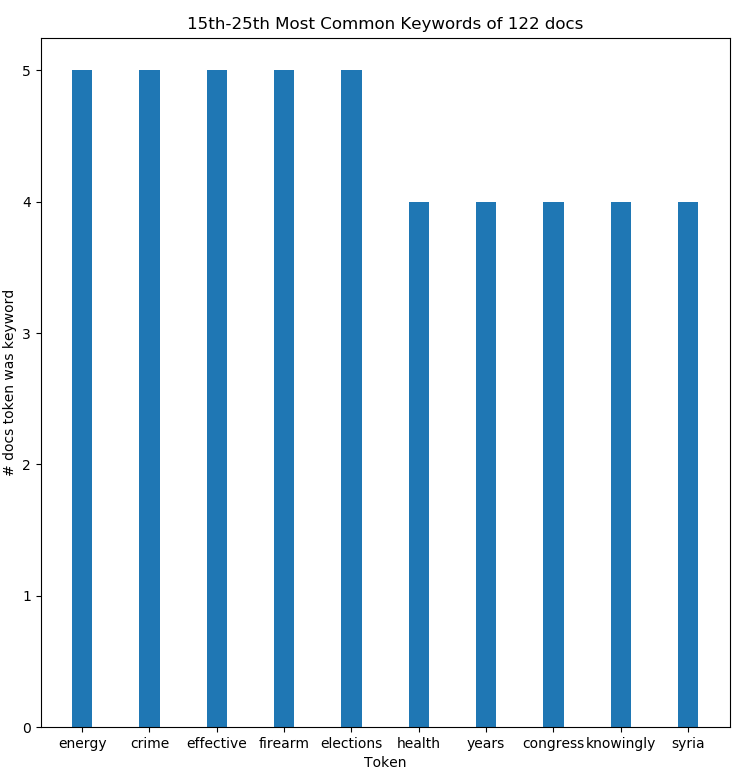
\includegraphics[scale=0.5]{test_kw-mostcommon_15-25}
  
  This graph represents the most common keywords of 122 documents. We will compare these with our summarizer to gauge our overall accuracy. We will also implement these key words in other ways such as creating word clouds and visual representations comparing our summarization to keyword accuracy. If time permits we also intend to implement sentiment visuals in our project that will be used in conjunction with these keywords.
  
  

\clearpage
\section{References}

[1] Los Angeles Times. (2011, June 19). Congress turns bill titles into acts of exaggeration. Retrieved from https://www.latimes.com/world/la-xpm-2011-jun-19-la-na-0620-titles-20110620-story.html 
\newline
\newline
[2] Moradi, M. (2018, November 13). CIBS: A biomedical text summarizer using topic-based sentence clustering. Retrieved from https://www.sciencedirect.com/science/article/pii/S1532046418302156?via=ihub 
\newline
\newline
[3] Kazantseva, A. (n.d.). Summarizing Short Stories. Retrieved from https://www.aclweb.org/anthology/J10-1003.pdf 
\newline
\newline
[4](n.d.). Retrieved from https://www.govinfo.gov/app/collection/crec/2020/01/01-10/6/{"pageSize":"20","offset":"0"} 

\end{document}
